\section{Simulation}
\subsection{Overview}

\begin{frame}{Simulation Overview}
    \mytwocolumn{0.6}{
        \begin{wideitemize}
            \item Simulation code preserved from CS257 submission.
            \item Simulates ``laminar flows of viscous, incompressible fluids''.
            \item Fluid is represented by a 2D array of cells.
            \item Fluid flows around static `obstacle' cells.
            \item Generates values for velocity $(u, v)$ and relative pressure $p$.
        \end{wideitemize}
    }{
        \begin{figure}
            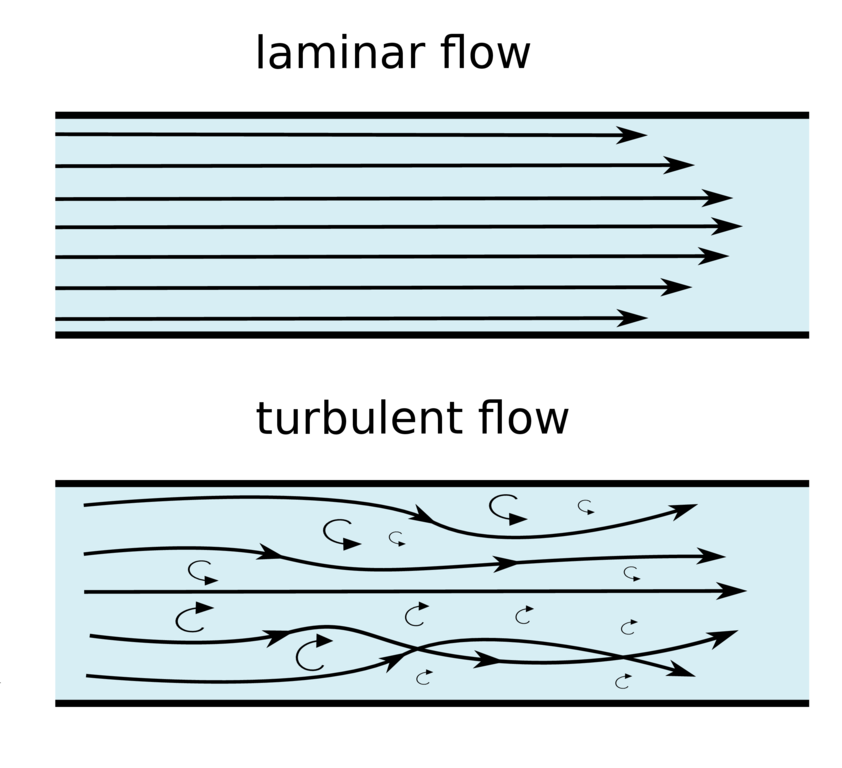
\includegraphics[width=\textwidth]{Presentation/images/sketch-laminar-flow-turbulent-flow.png}
            \caption{Laminar vs. turbulent fluid flow. Reproduced from cfdsupport.com}
            \label{fig:laminar_flow}
        \end{figure}
    }
\end{frame}

% \begin{frame}{Simulation Overview}
%     \mytwocolumn{0.6}{
%         \begin{wideitemize}
%             \item Simulation code preserved from CS257 submission.
%             \item 2D simulation of ``laminar flows of viscous, incompressible fluids''.
%             \item Generates values for velocity $(u, v)$ and relative pressure $p$.
%         \end{wideitemize}
%     }{
%         \input{FinalReport/Ch20Research/figures/staggered_grid}
%     }
% \end{frame}

\begin{frame}{Simulation Structure}
    \mytwocolumn{0.6}{
        \begin{wideitemize}
            \item Simulation runs in `ticks', each representing a discrete timestep $\delta{t}$.
            \item Each `tick' has multiple sequential execution stages.
            \item Each stage has been optimized to be embarassingly parallel.
            \item Poisson Solver runs for a constant amount of iterations each tick.
        \end{wideitemize}
    }{
        \begin{figure}
            \centering

        \begin{tikzpicture}[
        scale=0.8, every node/.style={scale=0.8},
        stage/.style={minimum height = 2.5em, draw, anchor=north}
        ]
            \newcommand{\stagesep}{-0.4};
            \node[stage](s1) at (0,0) {Compute $\delta{t}$};
            \node[stage](s2) at ($(s1.south) + (0,\stagesep)$) {Compute Tentative Velocity};
            \node[stage](s3) at ($(s2.south) + (0,\stagesep)$) {Compute Poisson RHS};
            \node[stage](s4) at ($(s3.south) + (0,\stagesep)$) {Poisson Solver};
            % \node[stage](s5) at ($(s4.south) + (0,-0.6)$) {Poisson Iteration \#2};
            % \node[stage](s6) at ($(s5.south) + (0,-0.6)$) {...};
            % \node[stage](s7) at ($(s6.south) + (0,-0.6)$) {Poisson Iteration \#N};
            \node[stage](s8) at ($(s4.south) + (0,\stagesep)$) {Update Velocity};
            \node[stage](s9) at ($(s8.south) + (0,\stagesep)$) {Boundary Conditions};

            \draw[thick, ->] (s4.east) arc (0:-330:-0.4cm);% syntax (starting point coordinates) arc (starting angle:ending angle:radius)
            \node at ($(s4.east) + (2cm, 0)$){$N$ {}iterations}; 

            \draw[-latex] (s1.south) -- (s2.north);
            \draw[-latex] (s2.south) -- (s3.north);
            \draw[-latex] (s3.south) -- (s4.north);
            \draw[-latex] (s4.south) -- (s8.north);
            % \draw[-latex] (s5.south) -- (s6.north);
            % \draw[-latex] (s6.south) -- (s7.north);
            % \draw[-latex] (s7.south) -- (s8.north);
            \draw[-latex] (s8.south) -- (s9.north);
        \end{tikzpicture}
        \caption{An example simulation tick}
        \label{fig:my_label}
    \end{figure}
    }
\end{frame}

\begin{frame}[fragile]{Simulation Kernels}
    % \begin{columns}\begin{column}{0.4\textwidth}
        \begin{wideitemize}
            \item This maps incredibly well to CUDA `kernels'\footnote{\url{https://docs.nvidia.com/cuda/cuda-c-programming-guide/index.html\#kernels}}.
            \item Each stage is implemented as one or more kernels, run over every element in parallel.
        \end{wideitemize}
    % \end{column}
    % \begin{column}{0.7\textwidth}
    \begin{figure}[b]
        \centering

        \lstset{language=c,keywords={__global__},
    keywordstyle=[1]\color{blue}}
        \begin{lstlisting}
// Computing delta-t is done slightly differently (ask me about it at the end!)
        
__global__ void computeTentativeVelocity_apply(...);
__global__ void computeTentativeVelocity_postproc_vertical(...);
__global__ void computeTentativeVelocity_postproc_horizontal(...);

__global__ void computeRHS_1per(...);

__global__ void poisson_single_tick(...);

__global__ void updateVelocity_1per(...);

__global__ void boundaryConditions_preproc_vertical(...);
__global__ void boundaryConditions_preproc_horizontal(...);
__global__ void boundaryConditions_apply(...);
__global__ void boundaryConditions_inputflow_west_vertical(...);\end{lstlisting}

        % \caption{CUDA Kernel Definitions}
    \end{figure}
    % \end{column}\end{columns}
\end{frame}

\begin{frame}{CUDA Unified Memory}
    % \todomark{Ask me about unified memory afterwards}
    
    \mytwocolumn{0.5}{
        \begin{wideitemize}
            \item CUDA provides Unified Memory allocations\footnotemark
            \item Paged between the Host and Device on-demand.
            \item Same performance as normal GPU memory when present on the device.
            \item Used to mix CPU and GPU implementations while testing and debugging.
        \end{wideitemize}
    }{
        \begin{figure}
            \centering
            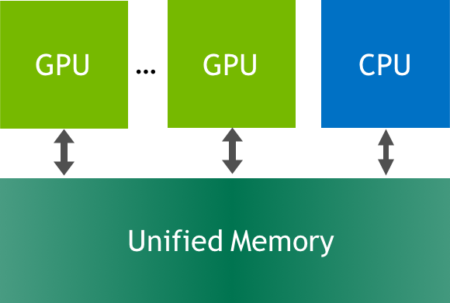
\includegraphics[width=0.7\textwidth]{Presentation/images/unified_memory_smol.png}
            % \caption{Caption}
            % \label{fig:my_label}
        \end{figure}
    }
    
    \footnotetext{\url{https://developer.nvidia.com/blog/unified-memory-cuda-beginners/}}
    
    % \vfill\null
    % \begin{center}
    %     Ask me about Simulation Memory Allocation at the end!
    % \end{center}
    % CUDA allows Unified Memory\parencite{https://developer.nvidia.com/blog/unified-memory-cuda-beginners/} to be allocated
    % Paged between Host and Device on-demand 
    % Allows incremental development of GPU kernels by using CPU code for kernels which haven't been ported yet.
    
    % image from {https://developer.nvidia.com/maximizing-unified-memory-performance-cuda-0}
\end{frame}

\subsection{Optimizations}

\begin{frame}[fragile]{\texttt{const \_\_restrict\_\_} pointers}
    % CUDA has a ``read-only data cache'' {https://docs.nvidia.com/cuda/cuda-c-programming-guide/index.html#global-memory-3-0}
    % Use `const __restrict__ T*` pointers to show the compiler which data is read-only
    % Developed a standardized kernel setup to ensure pointers are all __restrict__ed
    % Speeds up execution time\parencite{const restrict thingy}
    
    \begin{minipage}{0.5\textwidth}
        \begin{wideitemize}
        \item CUDA exposes a fast ``read-only data cache''\footnotemark{}.
        \item To ensure the compiler knows memory is read only, use the \texttt{const} and \texttt{\_\_restrict\_\_} qualifiers on all pointers.
        \item Shown to speed up execution times in \parencite{10.1145/3238147.3241533}.
        \end{wideitemize}
    \end{minipage}\hfill%
    \begin{minipage}{0.4\textwidth}
    \begin{figure}[b]
        \centering

        \lstset{language=c,keywords={template,typename,using},keywordstyle=[1]\color{blue}}
        \begin{lstlisting}
template<typename T>
using in_matrix = 
    const T* const __restrict__;

template<typename T>
using out_matrix = 
    T* const __restrict__;\end{lstlisting}
        \caption{Helper templates used in kernel definitions}
    \end{figure}
    \end{minipage}
    % }
    \footnotetext{\url{https://docs.nvidia.com/cuda/cuda-c-programming-guide/index.html\#global-memory-3-0}}
    
    \vfill\null
    \begin{center}
        Ask me about \texttt{const \_\_restrict\_\_} pointers at the end!
    \end{center}
    
    % Detail slide:
    % in_matrix<T> out_matrix<T>
    % Why out_matrix<T> needs to be __restrict__ too
\end{frame}

\begin{frame}{Parallel Reductions}
    % \todomark{Ask me about unified memory afterwards}
    
    \mytwocolumn{0.6}{
        \begin{wideitemize}
            \item Computing $\delta{t}$ requires the maximum values of $u, v$.
            \item We can do this in parallel on the GPU!
            \item Find the values on the GPU, then copy them to the CPU to calculate $\delta{t}$.
            \item Implementation taken from \parencite{CUDAParallelReduction}.
        \end{wideitemize}
    }{
        \begin{figure}
            \centering
            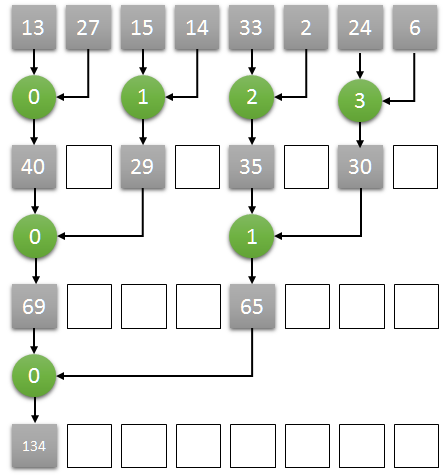
\includegraphics[width=0.7\textwidth]{Presentation/images/parallel_reduce.png}
            \caption{Example of parallel reduction for sum.\\Reproduced from \href{https://www.eximiaco.tech/en/2019/06/10/implementing-parallel-reduction-in-cuda/}{eximiaco.tech}}
            % \label{fig:my_label}
        \end{figure}
    }
    
    % \vfill\null
    % \begin{center}
    %     Ask me about Simulation Memory Allocation at the end!
    % \end{center}
    % CUDA allows Unified Memory\parencite{https://developer.nvidia.com/blog/unified-memory-cuda-beginners/} to be allocated
    % Paged between Host and Device on-demand 
    % Allows incremental development of GPU kernels by using CPU code for kernels which haven't been ported yet.
    
    % image from {https://developer.nvidia.com/maximizing-unified-memory-performance-cuda-0}
\end{frame}

\begin{frame}[fragile]{CUDA Graphs}
    % \todomark{Go in depth}
    % Profiling showed GPU bubbles between poisson iterations
    % cuda launches supposed to be asynchronous, but behaviour looks closer to synchronous
    % Instead of launching N times, record a CUDA graph containing N iterations, invoke that once.
    % Avoids CPU overhead, shows 2x speedup in profiler
    
    \begin{wideitemize}
        \item CPU overhead when launching Poisson kernels caused large GPU bubbles.
        \item Instead of launching N times, record a CUDA Graph\footnote{\url{https://developer.nvidia.com/blog/cuda-graphs/}} that runs N iterations, and launch it once.
        \item Theoretical 2x speedup.
    \end{wideitemize}
    
    \vfill\null
    \begin{minipage}{0.48\textwidth}
        \begin{lstlisting}
for (int i = 0; i < 100; i++) {
    launch poisson on stream;
}\end{lstlisting}
    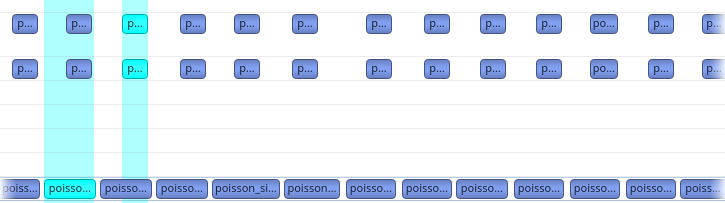
\includegraphics[width=\textwidth]{Presentation/images/cudagraphs_before.png}
    \begin{center}
        Individual Launches
    \end{center}
    \end{minipage}\hfill%
    \begin{minipage}{0.48\textwidth}
    \begin{lstlisting}
(record poisson100Iters if not present)

cudaGraphLaunch(poisson100Iters, stream);
\end{lstlisting}
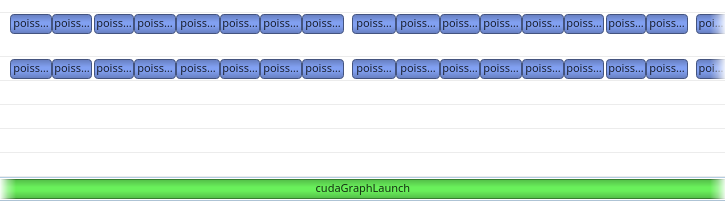
\includegraphics[width=\textwidth]{Presentation/images/cudagraphs_after.png}
        \begin{center}
        With CUDA Graphs
        \end{center}
    \end{minipage}
    % Potential cause
    % launches took more time than the actual execution
    % diminishing returns when kernels take longer

\end{frame}